\documentclass{article}
\usepackage[utf8]{inputenc}
\usepackage[T1]{fontenc}
\usepackage{booktabs}
\usepackage{caption}
\usepackage{graphicx}
\usepackage{multirow}
\usepackage{parskip}
\usepackage{hyperref}
\usepackage[a4paper, left=2cm, right=2cm, top=2cm, bottom=2cm]{geometry}

\newcommand{\tabitem}{~~\llap{\textbullet}~~}
\def \cmossensorinput {\texttt{cmos\_sensor\_input} }

\title{CMOS Sensor Input}
\author{Sahand Kashani}
\date{\today}

\begin{document}

\maketitle

\section{Core Overview}
The \cmossensorinput core is a highly configurable interface that makes it simple to connect a CMOS sensor to a host processor \& memory system.

The core is configurable at runtime through an Avalon Memory-Mapped (Avalon-MM) interface, and provides an Avalon Streaming (Avalon-ST) interface from the CMOS sensor.

It can be instantiated to accomodate various sensor pixel depths and sampling edges. Optionally, the core can also perform debayering and can pack multiple pixels together into a bigger word size in order to divide the required acquisition frequency and reduce pressure on the memory system.

The core comes with a set of C library interfaces that can be used to configure it and start its various operations.

\section{CMOS Sensors}
A CMOS sensor outputs 4 signals with which it is possible to sample its data:
\texttt{
    \begin{itemize}
        \itemsep-0.5em
        \item clock
        \item frame\_valid (1-bit)
        \item line\_valid (1-bit)
        \item data (n-bit)
    \end{itemize}
}

Figure~\ref{fig:cmos_sensor_signals_waveform} shows the relationship between the different signals for 2 frames that contains 2 rows and 3 columns each.

\begin{figure}[h]
    \centering
    \makebox[\textwidth][c]{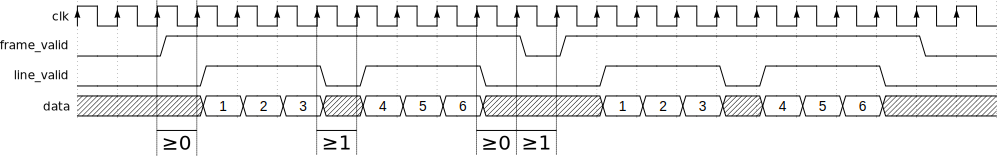
\includegraphics[width=1.0\textwidth]{fig/cmos_sensor_signals_waveform}}%
    \caption{CMOS sensor output signals for two $3\times2$ frames with a pixel depth of 3 bits. Spacing requirements between the various signals are specified in clock cycles.}
    \label{fig:cmos_sensor_signals_waveform}
\end{figure}

\newpage

\section{Block Diagram}
Figure~\ref{fig:cmos_sensor_input_external} shows a high-level view of the core, and Figure~\ref{fig:cmos_sensor_input_internal} shows the building blocks that compose it when in its \emph{largest} configuration (all optional units enabled, i.e. debayering unit and packer).

\begin{figure}[h]
    \centering
    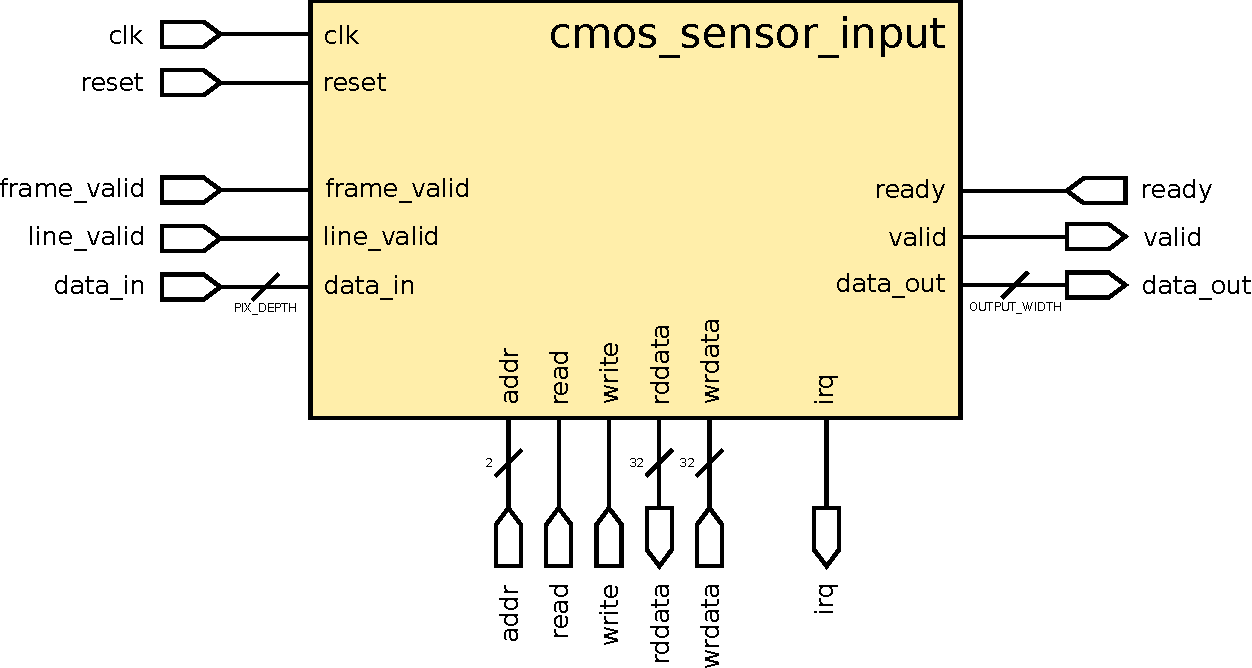
\includegraphics[width=0.75\textwidth]{fig/cmos_sensor_input_external}
    \caption{High-level block diagram.}
    \label{fig:cmos_sensor_input_external}
\end{figure}

The \cmossensorinput core is clocked by the \texttt{clock} output generated by the CMOS sensor and takes the \texttt{frame\_valid}, \texttt{line\_valid} and \texttt{data} signals as inputs.
Note that the \cmossensorinput core does \emph{not} need to be told what the dimensions of the incoming frame are. It solely relies on the \texttt{frame\_valid} and \texttt{line\_valid} signals to correctly acquire the data.

The core is composed of 7 components:

\begin{description}
    \item[\texttt{MM-Slave}] Provides an Avalon-MM slave interface from the unit to which a host processor can be connected. This interface allows the processor to submit commands and query the status of the unit.
    \item[\texttt{Synchronizer}] Captures all incoming signals from the CMOS sensor. The \texttt{synchronizer} can be parameterized to sample signals on the rising or falling edge of its input clock. The signals are synchronized by the \texttt{synchronizer} and are sent to the \texttt{sampler} on the next rising edge of the clock. All components of the \cmossensorinput core use the rising edge of the input clock for their operations.
    \item[\texttt{Sampler}] Acts as the valve on the stream of raw data coming from the sensor. It is responsible for determining the characteristics of the incoming frame supplied by the \texttt{synchronizer}, and, more importantly, for filtering and modifying the data and control signals to an internal format suitable for deterministic processing by the rest of the system.
    \item[\texttt{Debayer}] Applies a $3\times3$ debayering pattern over the incoming frame supplied by the \texttt{sampler}. The debayering pattern used can be configured at runtime to accomodate for the 4 possible pixel layouts of any sensor.
    \item[\texttt{Packer}] Packs consecutive pixels received from the previous stage into a larger word. When no more pixels can be packed in the output word size, then the word is sent out of the unit.
    \item[\texttt{SC\_FIFO}] Buffer that stores data ready to be sent out of the unit.
    \item[\texttt{ST-Source}] Provides an Avalon-ST source interface from the unit. The unit supports backpressure due to the presence of the \texttt{ready} port.
\end{description}

\begin{figure}[h!]
    \centering
    \makebox[\textwidth][c]{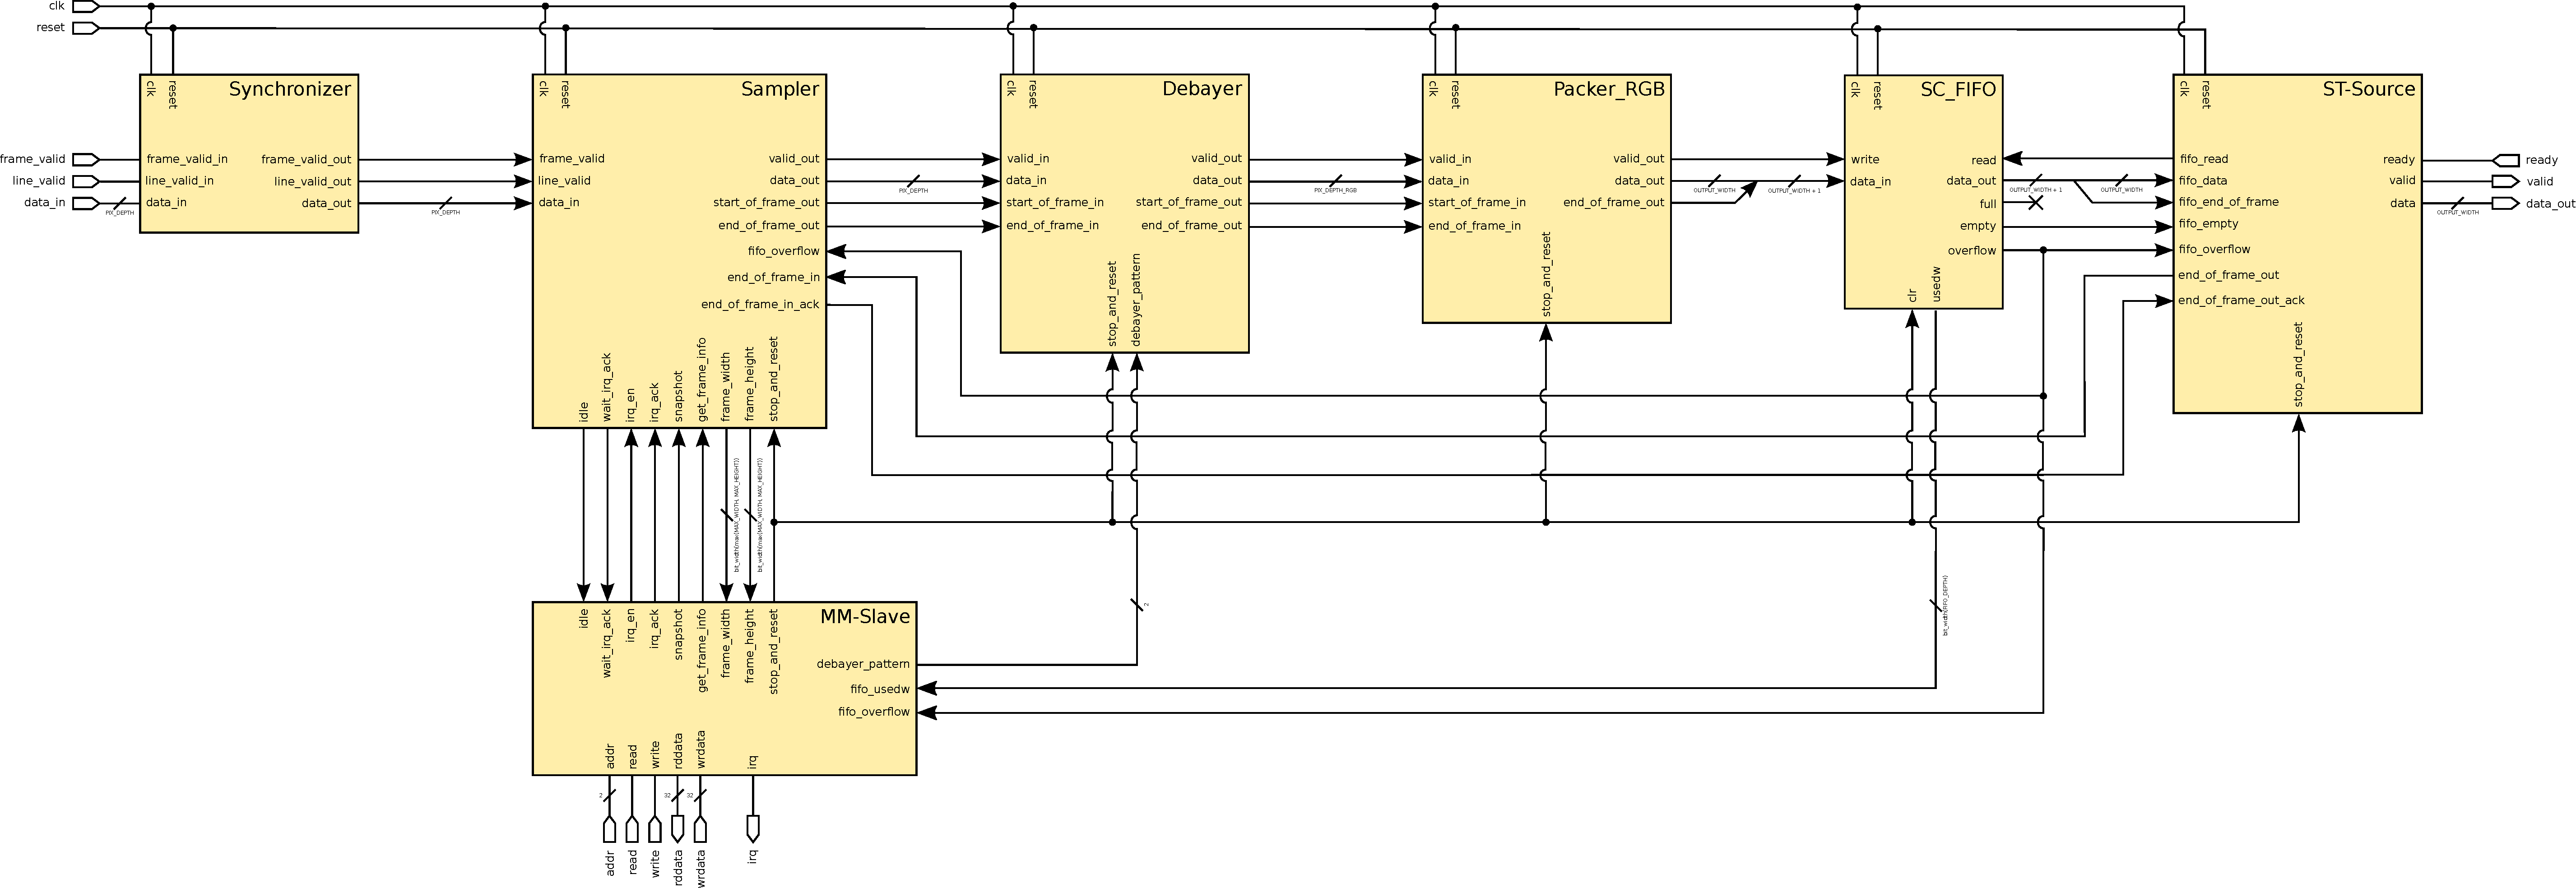
\includegraphics[width=0.9\textheight,angle=90]{fig/cmos_sensor_input_internal}}%
    \caption{Internal block diagram.}
    \label{fig:cmos_sensor_input_internal}
\end{figure}

\newpage

\section{Qsys Interface}
Figure~\ref{fig:qsys_gui} shows the Qsys configuration interface for the core.
\begin{figure}[h]
    \centering
    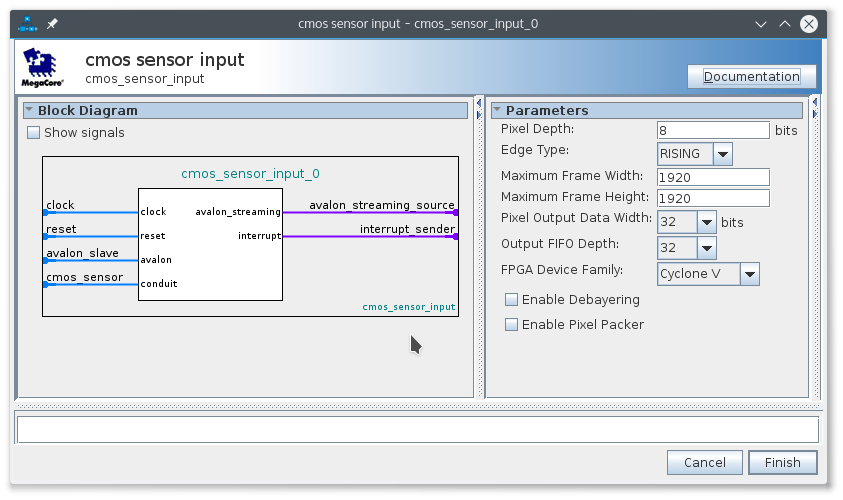
\includegraphics[width=0.9\textwidth]{fig/qsys_gui}
    \caption{Qsys Configuration Interface.}
    \label{fig:qsys_gui}
\end{figure}

It can be configured through 9 parameters, shown in Table~\ref{tab:core_parameters}.

\begin{table}[h]
    \centering
    \texttt{
        \begin{tabular}{lccc}
            \toprule
            Parameter       & Type     & Values                      & Default Value \\
            \midrule
            PIX\_DEPTH      & Positive & 1, 2, 3, ..., 32            & 8             \\
            SAMPLE\_EDGE    & String   & "RISING", "FALLING"         & "RISING"      \\
            MAX\_WIDTH      & Positive & 2, 3, 4, ..., 65535         & 1920          \\
            MAX\_HEIGHT     & Positive & 1, 2, 3, ..., 65535         & 1080          \\
            OUTPUT\_WIDTH   & Positive & 8, 16, 32, ..., 1024        & 32            \\
            FIFO\_DEPTH     & Positive & 8, 16, 32, ..., 1024        & 32            \\
            DEVICE\_FAMILY  & String   & "Cyclone V", "Cyclone IV E" & "Cyclone V"   \\
            DEBAYER\_ENABLE & Boolean  & FALSE, TRUE                 & FALSE         \\
            PACKER\_ENABLE  & Boolean  & FALSE, TRUE                 & FALSE         \\
            \bottomrule
        \end{tabular}
    }
    \caption{Controller register map. All registers are \texttt{32} bits wide.}
    \label{tab:core_parameters}
\end{table}

Some general notes about the possible parameter values:
\begin{itemize}
    \item \texttt{PIX\_DEPTH} is arbitraily restricted to go until 32 bits, but it can be increased without any design changes.
    \item \texttt{MAX\_WIDTH} and \texttt{MAX\_HEIGHT} are restricted to 65535 due to the Avalon-MM slave interface. The data width is 32 bits, and both the frame's current width and height take up 16 bits of a common \texttt{FRAME\_INFO} register when read, so their maximum value is restricted to 65535. If the width of the Avalon-MM slave is increased, then the maximum width and height can take much larger values.
    \item \texttt{MAX\_HEIGHT} can go down to as low as 1 row, however \texttt{MAX\_WIDTH} can only go down to 2 colums. As such, the minimum capturable frame is of \texttt{2x1}. This restriction is in place to avoid the \texttt{start\_of\_frame} and \texttt{end\_of\_frame} signals used between the various components from overlapping. This also ensures that at least 2 pixels fit in a packed word (so the \texttt{packer} actually is useful).
    \item \texttt{OUTPUT\_WIDTH} is the bit width of an Avalon-ST interface, and therefore must be a multiple of 8. The possible values are arbitrarily limited to powers of 2 instead to make the list of suggested values short in the Qsys GUI. If this requirement causes issues for your designs, you can modify the Qsys file describing the component to allow non-power of two values (as long as they remain multiples of 8).
    \item \texttt{FIFO\_DEPTH} must be a power of two for technology reasons.
    \item \texttt{DEVICE\_FAMILY} is needed to choose the appropriate implementation of the FIFO for the intended target device. Currently, this parameter only supports \texttt{"Cyclone V"} and \texttt{"Cyclone IV E"} as values. However, this choice was arbitary in the sense that they are the only devices on which the unit was tested. There is actually no restriction involved, and any other family should also work if you need to target another device.
\end{itemize}

\section{Components}
\subsection{MM-Slave}
Table~\ref{tab:register_map} shows the register map exposed by the Avalon-MM slave interface.

\begin{table}[h]
    \centering
    \texttt{
        \begin{tabular}{ccc}
            \toprule
            Offset & Type & Name        \\
            \midrule
            0x00   & RW   & CONFIG      \\
            0x04   & WO   & COMMAND     \\
            0x08   & RO   & STATUS      \\
            0x0C   & RO   & FRAME\_INFO \\
            \bottomrule
        \end{tabular}
    }
    \caption{Avalon-MM slave register map. All registers are \texttt{32} bits wide.}
    \label{tab:register_map}
\end{table}

\subsubsection{\texttt{CONFIG} register}
The unit is configured through its \texttt{CONFIG} register, shown in Table~\ref{tab:config_register}.

\begin{table}[h]
    \centering
    \texttt{
        \begin{tabular}{cccc}
            \toprule
            Bit  & Name             & Value & Description       \\
            \midrule
            31:3 & reserved         & N/A   & N/A               \\
            2:1  & DEBAYER\_PATTERN & 0     & RGGB              \\
                 &                  & 1     & BGGR              \\
                 &                  & 2     & GRBG              \\
                 &                  & 3     & GBRG              \\
            0    & IRQ              & 0     & Interrupt disable \\
                 &                  & 1     & Interrupt enable  \\
            \bottomrule
        \end{tabular}
    }
    \caption{\texttt{CONFIG} register definitions. Note that the \texttt{CONFIG} register can only be modified when the core is in the \texttt{IDLE} state.}
    \label{tab:config_register}
\end{table}

If the \texttt{IRQ} bit is set, then interrupts are generated for successful \texttt{GET\_FRAME\_INFO} and \texttt{SNAPSHOT} commands, and upon FIFO overflows.

\subsubsection{\texttt{COMMAND} register}

Commands are submitted to the unit through its \texttt{COMMAND} register, shown in Table~\ref{tab:command_register}.

\begin{table}[h]
    \centering
    \texttt{
        \begin{tabular}{ccl}
            \toprule
            Name             & Value & Description                                       \\
            \midrule
            GET\_FRAME\_INFO & 0     & Analyze a frame to determine its width and height \\
            SNAPSHOT         & 1     & Capture a frame                                   \\
            IRQ\_ACK         & 2     & Acknowledge interrupt                             \\
            STOP\_AND\_RESET & 3     & Stop sampler and reset all other units            \\
            \bottomrule
        \end{tabular}
    }
    \caption{\texttt{COMMAND} register definitions.}
    \label{tab:command_register}
\end{table}

\subsubsection{\texttt{STATUS} register}

The unit's current state can be read through its \texttt{STATUS} register, shown in Table~\ref{tab:status_register}.

\begin{table}[h]
    \centering
    \texttt{
        \begin{tabular}{cccc}
            \toprule
            Bit   & Name           & Value         & Description     \\
            \midrule
            31:13 & reserved       & N/A           & N/A             \\
            12:2  & FIFO\_USEDW    & 0:FIFO\_DEPTH & FIFO fill level \\
            1     & FIFO\_OVERFLOW & 0             & NO\_OVERFLOW    \\
                  &                & 1             & OVERFLOW        \\
            0     & STATE          & 0             & Idle            \\
                  &                & 1             & Busy            \\
            \bottomrule
        \end{tabular}
    }
    \caption{\texttt{STATUS} register definitions.}
    \label{tab:status_register}
\end{table}

\subsubsection{\texttt{FRAME\_INFO} register}
Information about the analyzed frame (as observed by the unit when the \texttt{GET\_FRAME\_INFO} was submitted) can be read through the unit's \texttt{FRAME\_INFO} register, shown in Table~\ref{tab:frame_info_register}.

\begin{table}[h]
    \centering
    \texttt{
        \begin{tabular}{cccc}
            \toprule
            Bit   & Name          & Value           & Description           \\
            \midrule
            31:16 & FRAME\_HEIGHT & {1:MAX\_HEIGHT} & Observed frame height \\
            15:0  & FRAME\_WIDTH  & {2:MAX\_WIDTH}  & Observed frame width  \\
            \bottomrule
        \end{tabular}
    }
    \caption{\texttt{FRAME\_INFO} register definitions.}
    \label{tab:frame_info_register}
\end{table}

\subsection{Sampler}
The \texttt{sampler} is the most complicated component of the \cmossensorinput core, as can be seen by its state machine diagram, shown in Figure~\ref{fig:sampler_state_machine}.

The \texttt{sampler}'s main task is to transform the CMOS sensor's signals to the format shown in Figure~\ref{fig:sampler_waveform}.

\begin{figure}[h!]
    \centering
    \makebox[\textwidth][c]{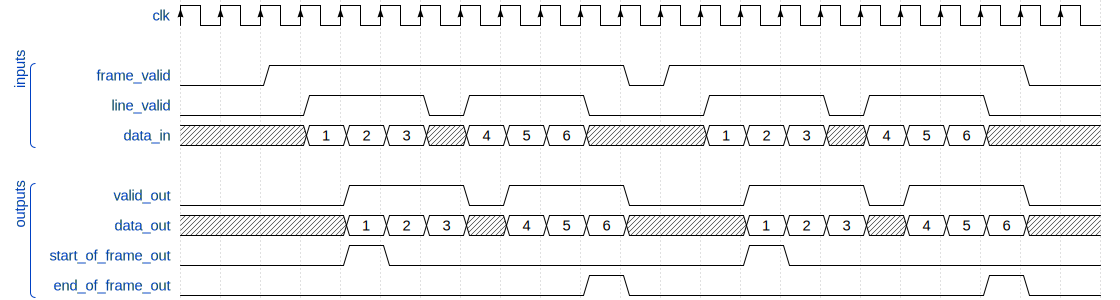
\includegraphics[width=1.0\textwidth]{fig/sampler_waveform}}%
    \caption{Sampler output data format.}
    \label{fig:sampler_waveform}
\end{figure}

Note that \texttt{start\_of\_frame}  (respectively, \texttt{end\_of\_frame}) must be generated on the first (respectively, last) cycle where \texttt{data\_out} is valid. It must \emph{not} be generated before (respectively, after) the \texttt{valid} signal is asserted (respectively, deasserted).

In order to satisfy these timing constraints, the \texttt{sampler} needs to know the incoming frame width and height in advance. However, we want to avoid the user of the \cmossensorinput core from having to manually program the frame dimensions through the Avalon-MM slave interface each time the core is used.

To get around this issue, we instead provide a \texttt{GET\_FRAME\_INFO} command. By submitting this command to the core, you instruct the \texttt{sampler} to analyze a frame flowing through it in order to automatically determine the frame dimensions. Note that the \texttt{sampler} does not perform any outputting when analyzing a frame. Outputting is only done upon reception of a \texttt{SNAPSHOT} command.

\begin{figure}[h!]
    \centering
    \makebox[\textwidth][c]{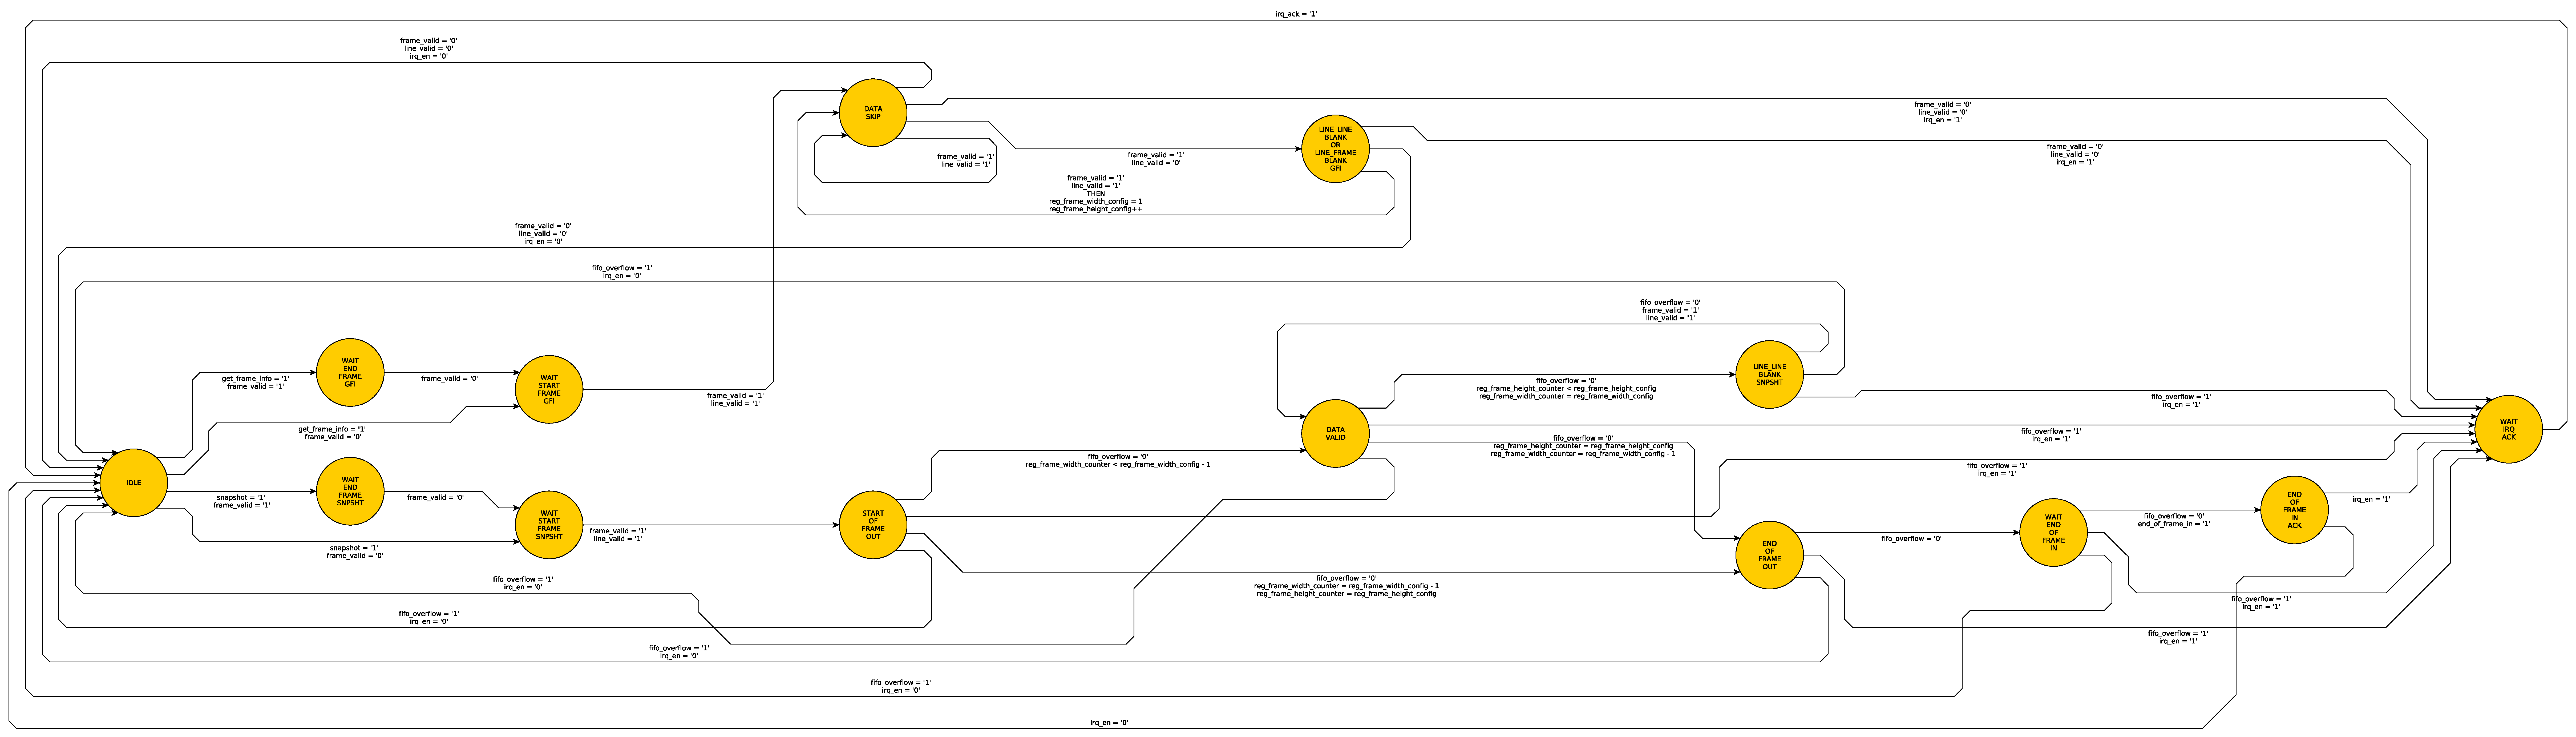
\includegraphics[width=0.9\textheight,angle=90]{fig/sampler_state_machine}}%
    \caption{Sampler state machine. For legibility, the diagram does not show the outputs at each state, or the synchronous reset transition from all states back to the \texttt{IDLE} state upon receiving \texttt{stop\_and\_reset}.}
    \label{fig:sampler_state_machine}
\end{figure}

Note that the \texttt{sampler} stops immediately upon a FIFO overflow to allow the host to reconfigure the core.

\newpage

\subsection{Debayer}
% TODO : insert future state machine
\emph{The \texttt{debayer} unit is currently unimplemented. If enabled, it will simply copy its input to its output (appropriately resizing data to match the required bit widths). As such, please do not enable this option at this this time. This unit will be implemented in a future revision of the \cmossensorinput core.}

\subsection{Packer}
The \texttt{packer} essentially consists of a shift-register. Incoming data is shifted in from the right until as many pixels that the data width supports are received. The remaining bits are filled with zeros. Figures~\ref{fig:packer_waveform} and \ref{fig:packer_waveform2} show the behaviour of the \texttt{packer} for different configurations.

\begin{figure}[h!]
    \centering
    \makebox[\textwidth][c]{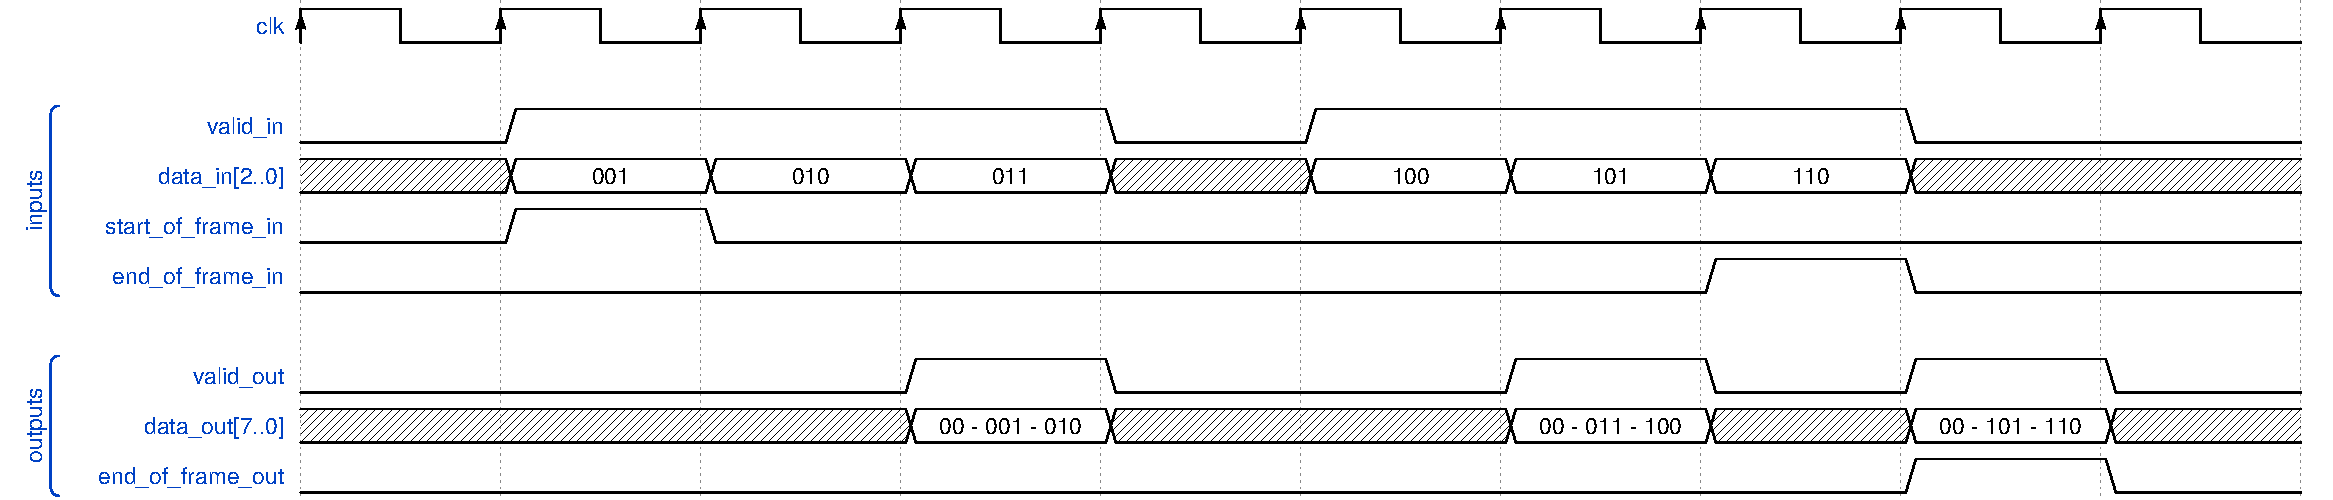
\includegraphics[width=1.0\textwidth]{fig/packer_waveform}}%
    \caption{Packer waveform for two consecutive $3\times2$ frames (\texttt{PIX\_DEPTH = 3}, \texttt{OUTPUT\_WIDTH = 8}).}
    \label{fig:packer_waveform}
\end{figure}

\begin{figure}[h!]
    \centering
    \makebox[\textwidth][c]{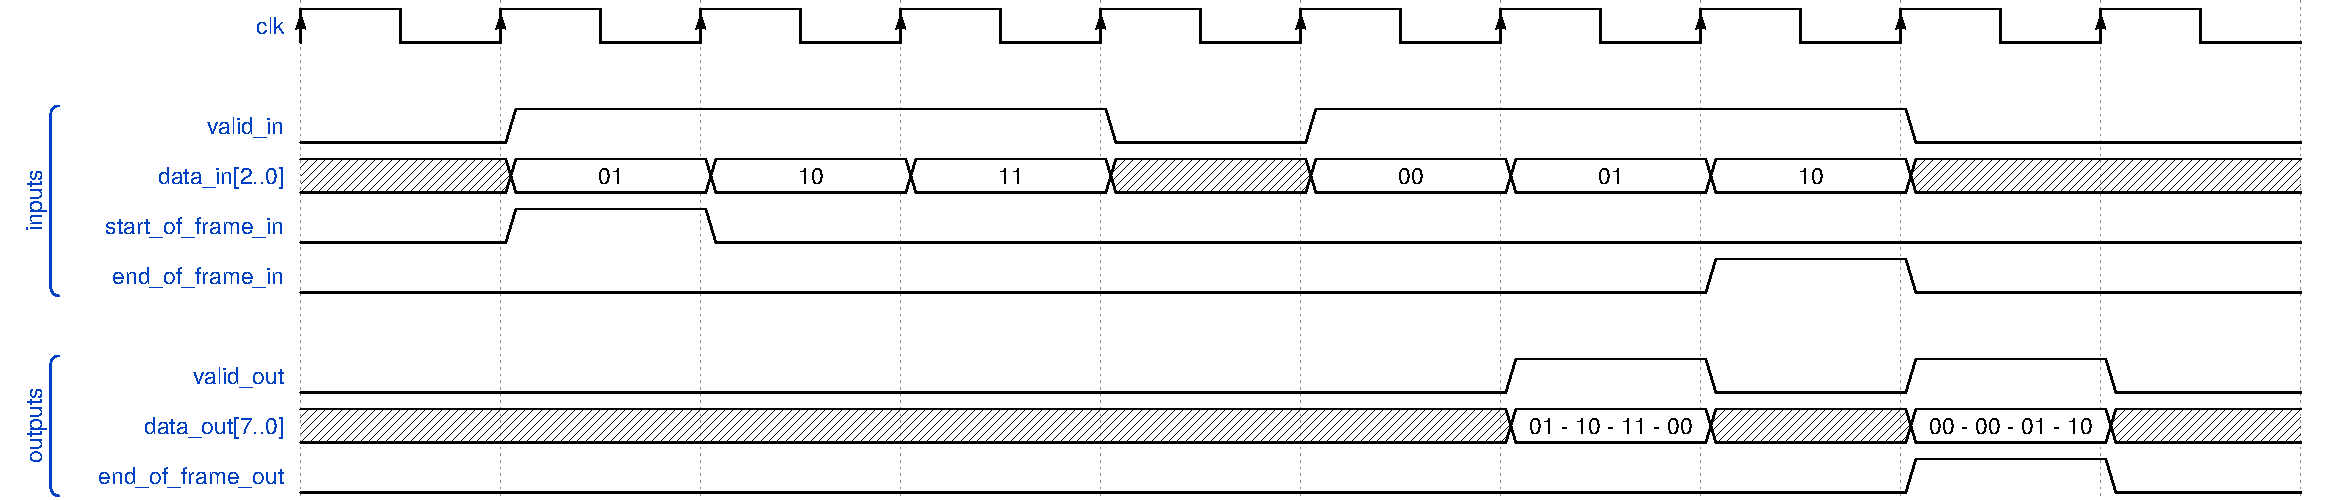
\includegraphics[width=1.0\textwidth]{fig/packer_waveform2}}%
    \caption{Packer waveform for two consecutive $3\times2$ frames (\texttt{PIX\_DEPTH = 2}, \texttt{OUTPUT\_WIDTH = 8}).}
    \label{fig:packer_waveform2}
\end{figure}

\subsection{SC\_FIFO}
This component consists of a single-clocked FIFO that holds the output of the \cmossensorinput core until it is sent out of the unit. It is actually a \emph{wrapper} around a specific FIFO implementation depending on the device family the design is instantiated on.

In Figure~\ref{fig:cmos_sensor_input_internal}, we see that the \texttt{empty} output is used downstream by the \texttt{ST-Source} component to know if the FIFO can be read.
However, the \texttt{full} output is not used upstream by the \texttt{packer} to avoid writing to a full FIFO.
This is not an issue, as write protection is implemented within the \texttt{sc\_fifo} component itself, and external units do not need to test before writing.
This is done to centralize write protection to a single place (since the core is modular and components can be moved around).

If the FIFO overflows, then you must submit a \texttt{STOP\_AND\_RESET} command to reinitialize the device.

\section{Extensibility}
The core is versatile: it is possible to add any additional filters needed for your application between the \texttt{sampler} and the \texttt{packer}. The only requirement is that \emph{all} components placed between these two points use the same data format outputted by the \texttt{sampler} for their inputs \emph{and} outputs. This is required so that different elements can be easily reordered and composed.

For example, one can add any convolutional filter after the \texttt{debayer} unit.

\end{document}
